\newpage\BorderFirstPage
\chapter[~]{Вивчення додаткових можливостей креслення в системі КОМПАС-3D}

\textbf{Мета роботи} --- ознайомитись з додатковими прийомами виконання креслень в програмному
пакеті підготовки конструкторської документації КОМПАС-3D, навчитись виконувати креслення
ускладнених деталей на площині.

\section{Виконання роботи}

Згідно з варінтом для побудови була задана наступна деталь:

\begin{figure}[!ht]
  \centering 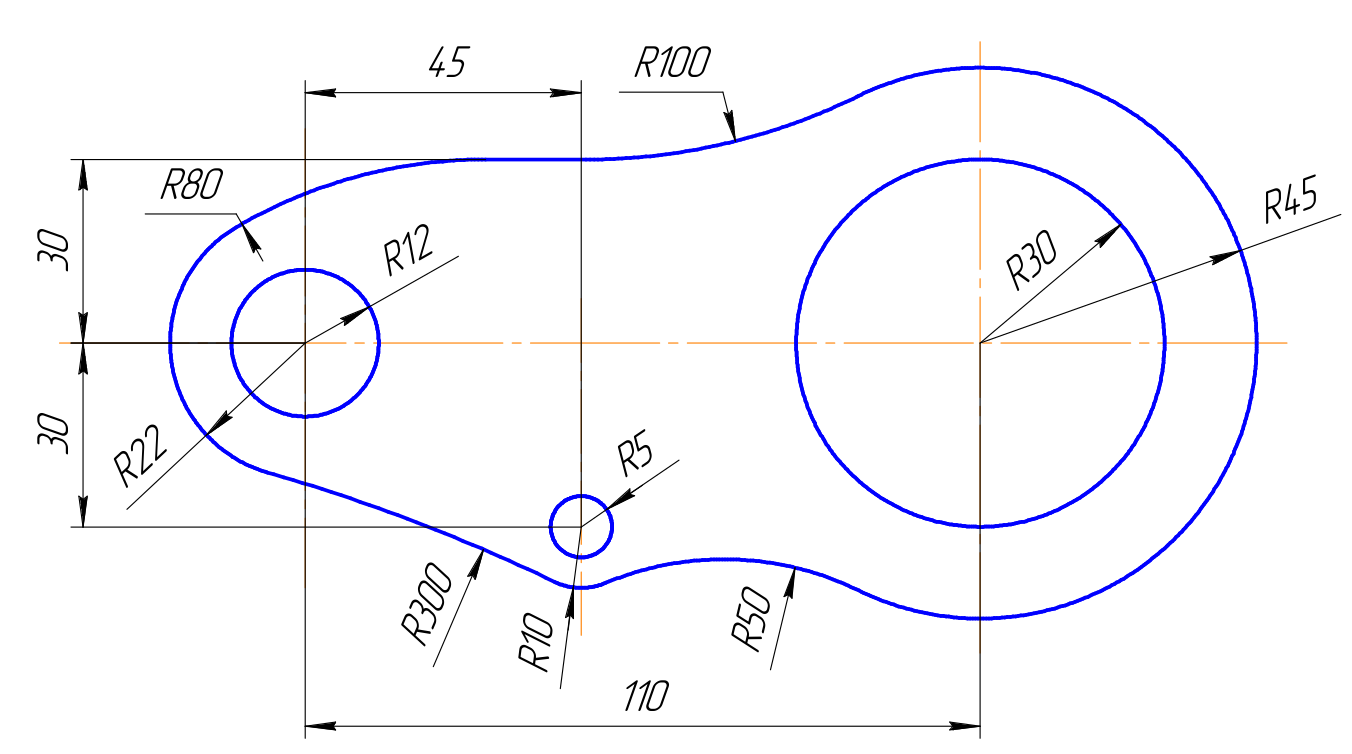
\includegraphics[width=0.9\linewidth]{./images/lab4/target_drawing.png}
  \caption{Задана деталь для побудови}
  \label{fig:lab3:target_part} 
\end{figure}
\FloatBarrier

\begin{enumerate}[leftmargin=*]
\item Створюємо новий шар (\ref{fig:lab4:new_layer}) на якому буде знаходитись допоміжна геометрія,
  яку можна буде в процесі приховати, без ручного видалення допоміжних елементів. Основне креслення
  буде знаходитись в \textit{системному шарі}.

  \newpage\restoregeometry\BorderText
  \begin{figure}[!ht]
    \centering 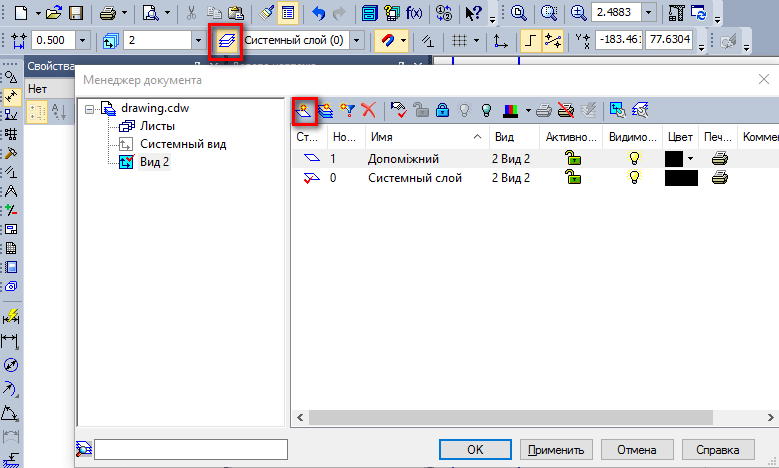
\includegraphics[width=0.9\linewidth]{./images/lab4/create_new_layer.png}
    \caption{Створення новго шару.}
    \label{fig:lab4:new_layer}
  \end{figure}
  \FloatBarrier

\item Створюємо два кола на на кординатах (0, 0) та (0, -110) та проводимо між центрами цих кіл
  осьову лінію з координатами (0,-110) та (0,50). Додаємо допоміжну точку на координатах (0,
  -65). (\ref{fig:lab4:step1}).
  \begin{figure}[!ht]
    \centering 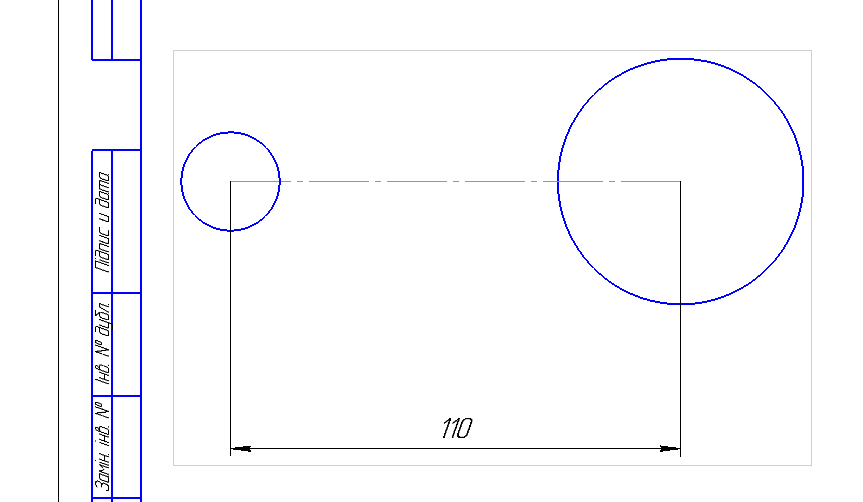
\includegraphics[width=0.9\linewidth]{./images/lab4/step1.png}
    \caption{\label{fig:lab4:step1}}
  \end{figure}
  \FloatBarrier

\item Задаємо розміри для побудованих елементів (\ref{fig:lab4:step2}).
  \begin{figure}[!ht]
    \centering 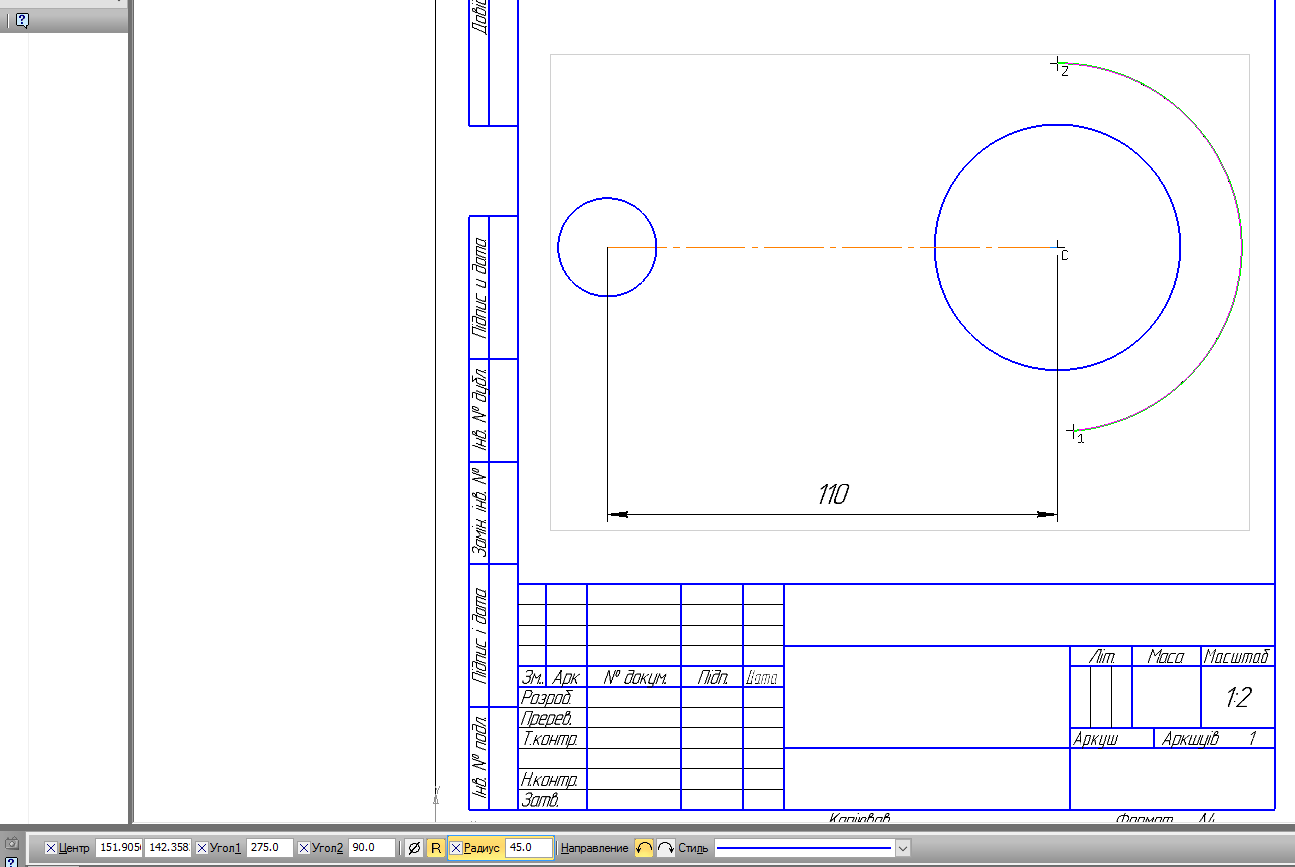
\includegraphics[width=0.9\linewidth]{./images/lab4/step2.png}
    \caption{\label{fig:lab4:step2}}
  \end{figure}
  \FloatBarrier

\item Будуємо коло радіосом 5 мм та центром (-65 -30), опускаємо до нього тонкі лінії. Вставнолюємо
  точку з кординатами (-65, 30) в допоміжно шарі (\ref{fig:lab4:step3}).
  \begin{figure}[!ht]
    \centering 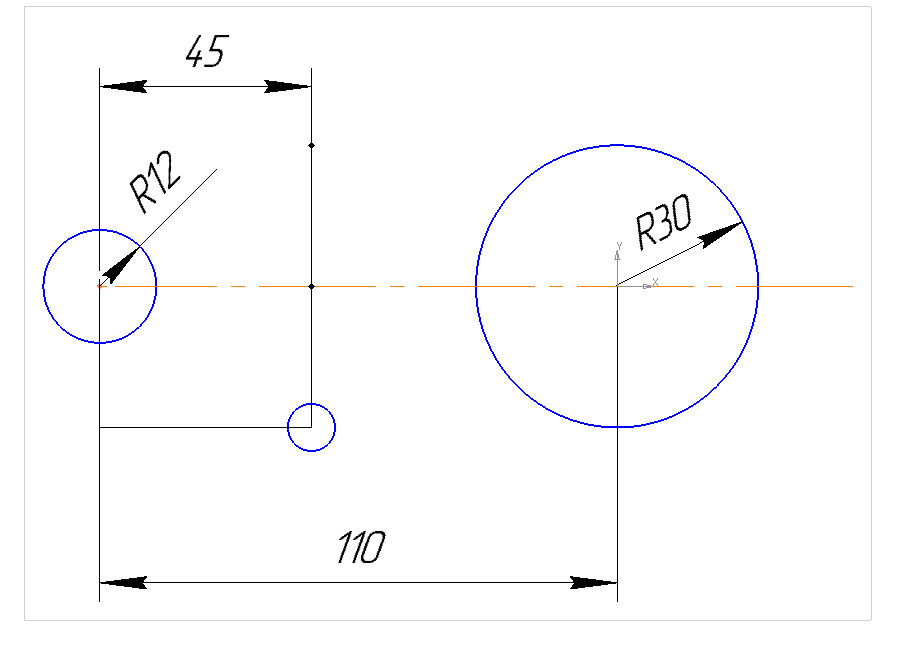
\includegraphics[width=0.7\linewidth]{./images/lab4/step3.png}
    \caption{\label{fig:lab4:step3}}
  \end{figure}
  \FloatBarrier

\item Позначаємо розміри для побудованих елементів (\ref{fig:lab4:step4}).
  \begin{figure}[!ht]
    \centering 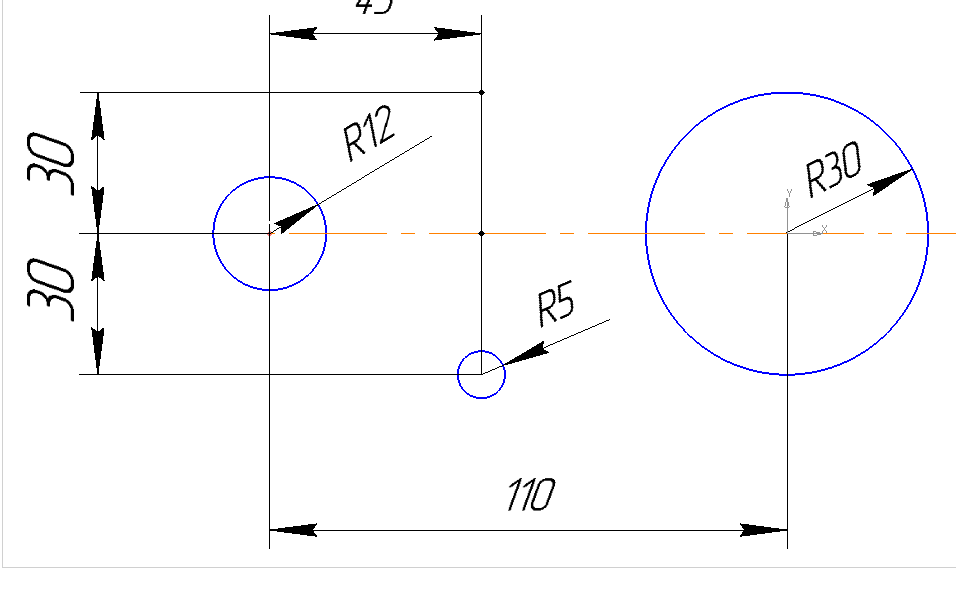
\includegraphics[width=0.9\linewidth]{./images/lab4/step4.png}
    \caption{\label{fig:lab4:step4}}
  \end{figure}
  \FloatBarrier

\item Будуємо дугу радіусом 45мм та позначаємо її радіальний діаметр (\ref{fig:lab4:step5}).
  \begin{figure}[!ht]
    \centering 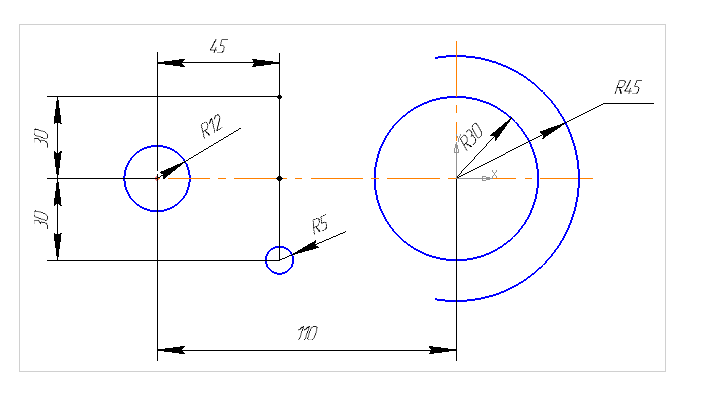
\includegraphics[width=0.9\linewidth]{./images/lab4/step5.png}
    \caption{\label{fig:lab4:step5}}
  \end{figure}
  \FloatBarrier
  
\item Будуємо дуги радіусами 100мм, 80мм та 22 мм відповідно (\ref{fig:lab4:step6}).
  \begin{figure}[!ht]
    \centering 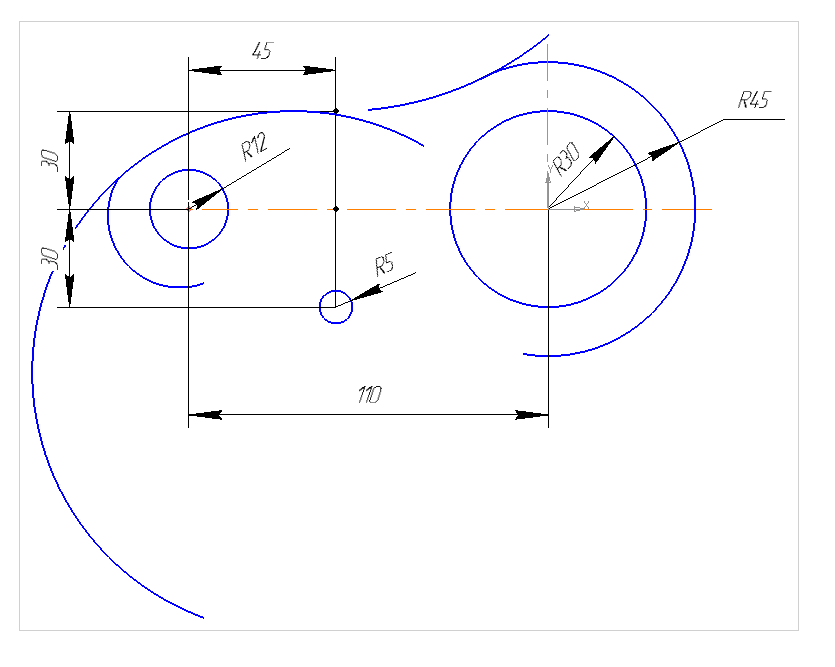
\includegraphics[width=0.7\linewidth]{./images/lab4/step6.png}
    \caption{\label{fig:lab4:step6}}
  \end{figure}
  \FloatBarrier

\item \label{item:cut_curve}За допомогою інструменту ``Відсікти криву'' \textit{(``Усечь кривую'')}
  видалямо частини що періскаються для дуг R100 та R45 (\ref{fig:lab4:step7}).
  \begin{figure}[!ht]
    \centering 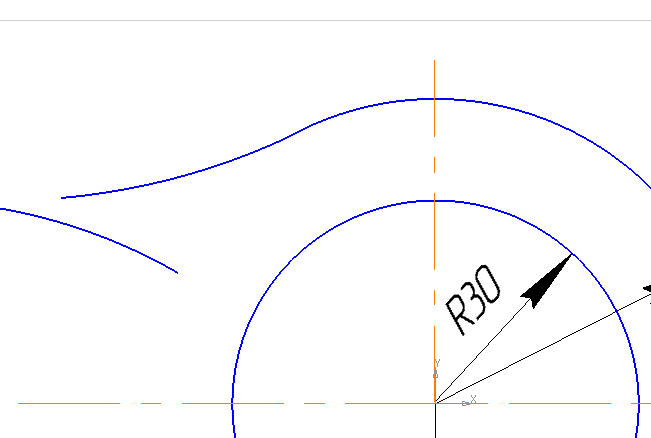
\includegraphics[width=0.9\linewidth]{./images/lab4/step7.png}
    \caption{\label{fig:lab4:step7}}
  \end{figure}
  \FloatBarrier

\item \label{item:round} За допомогою інструменту ``Заокруглення''(``Скругление'') закоруглюємо
  редаговані дуги (\ref{fig:lab4:step8}).
  \begin{figure}[!ht]
    \centering 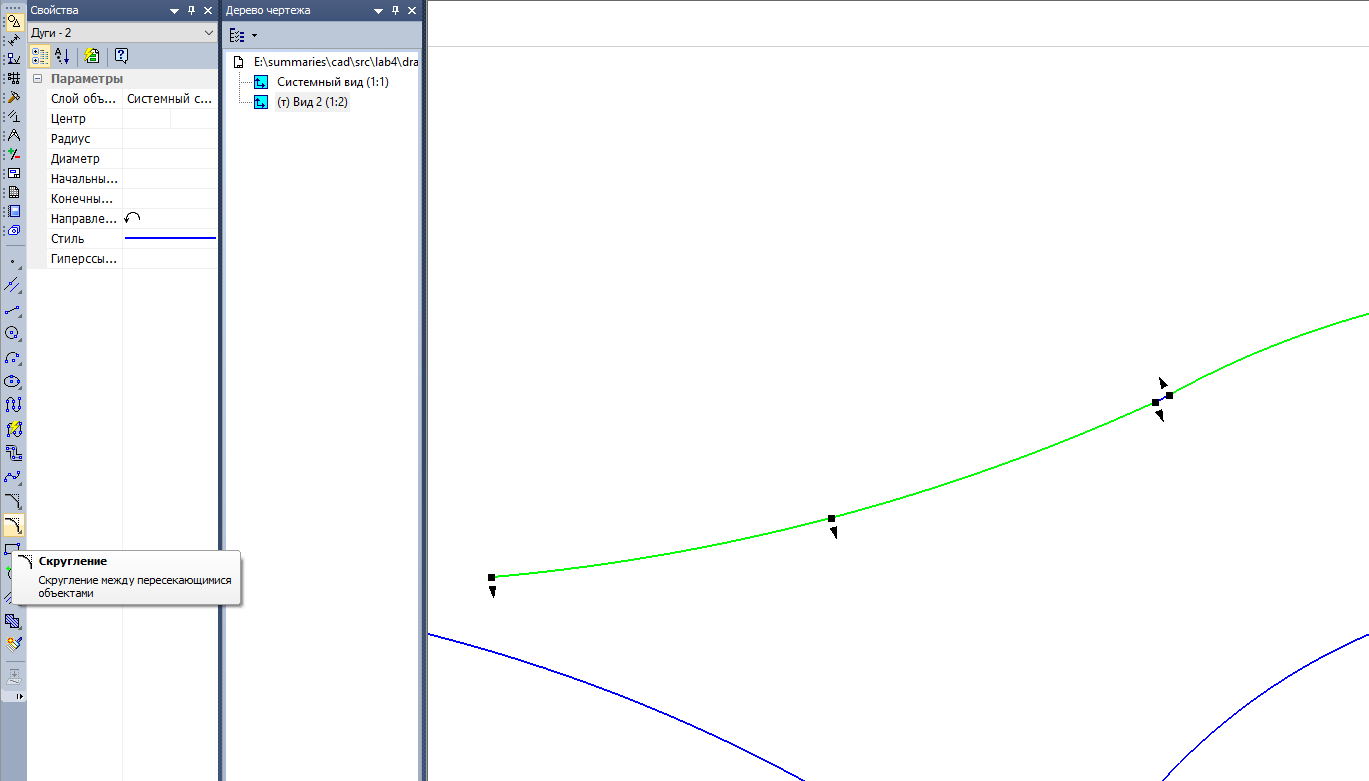
\includegraphics[width=0.9\linewidth]{./images/lab4/step8.png}
    \caption{\label{fig:lab4:step8}}
  \end{figure}
  \FloatBarrier

\item Добудовуємо дуги R300, R10 та R50.  (\ref{fig:lab4:step9}).
  \begin{figure}[!ht]
    \centering 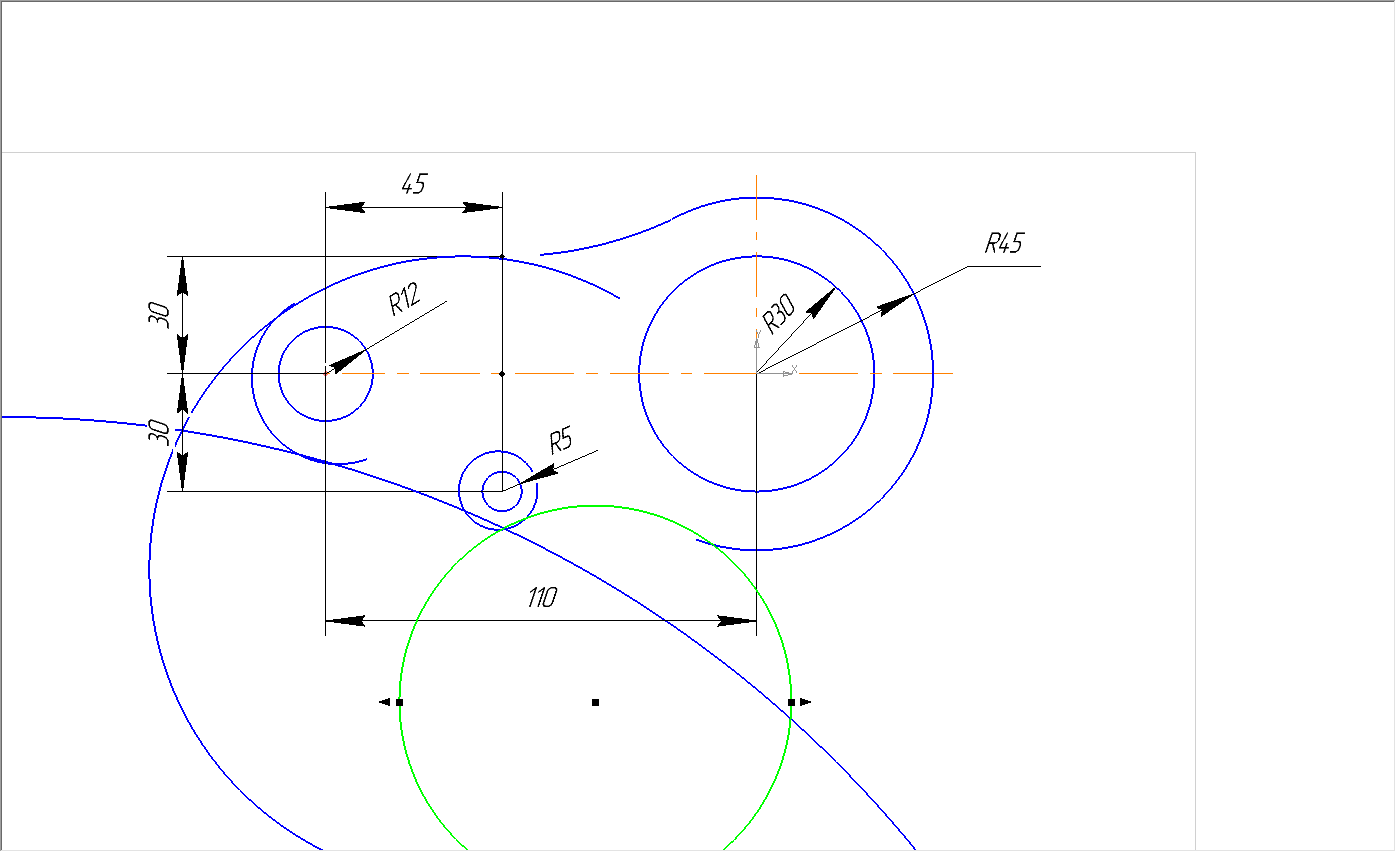
\includegraphics[width=0.9\linewidth]{./images/lab4/step9.png}
    \caption{\label{fig:lab4:step9}}
  \end{figure}
  \FloatBarrier

\item Для побудованих кривих проводимо ті ж операції, що і на кроках \ref{item:cut_curve} ---
  \ref{item:round}.  (\ref{fig:lab4:step10}).
  \begin{figure}[!ht]
    \centering 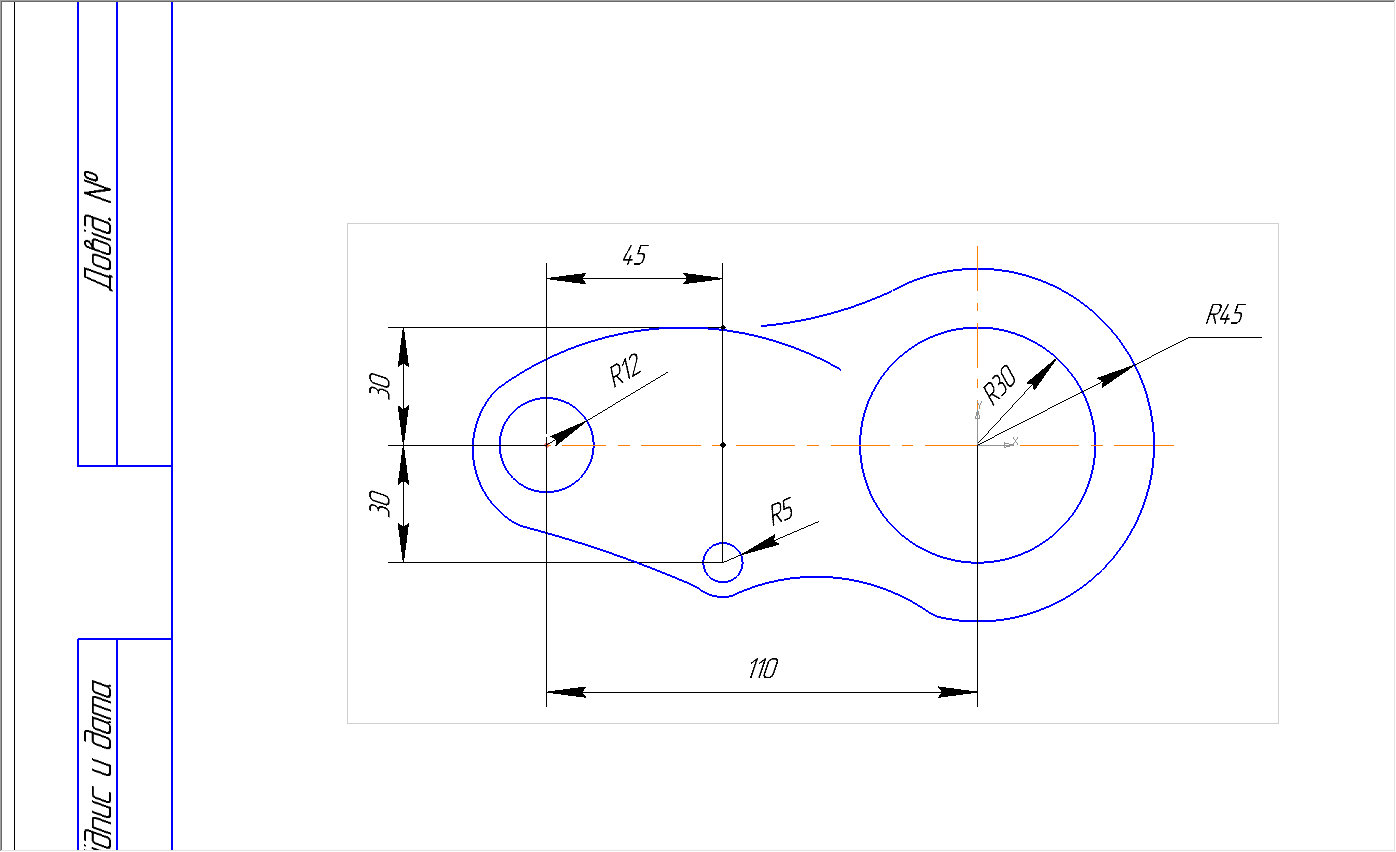
\includegraphics[width=0.9\linewidth]{./images/lab4/step10.png}
    \caption{\label{fig:lab4:step10}}
  \end{figure}
  \FloatBarrier

\item Вимикаємо видимість допоміжного шару, щоб сховати непотрібну допоміжну
  геометрію. (\ref{fig:lab4:step11}).
  \begin{figure}[!ht]
    \centering 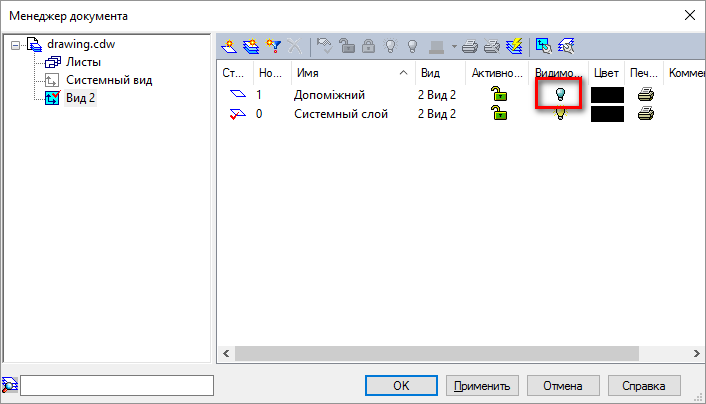
\includegraphics[width=0.9\linewidth]{./images/lab4/step11.png}
    \caption{\label{fig:lab4:step11}}
  \end{figure}
  \FloatBarrier
  
\end{enumerate}

Готовий кресленик навадений на сторінці \pageref{lab4:pdf:drawing}.
\newpage
\NoBorder
\label{lab4:pdf:drawing}
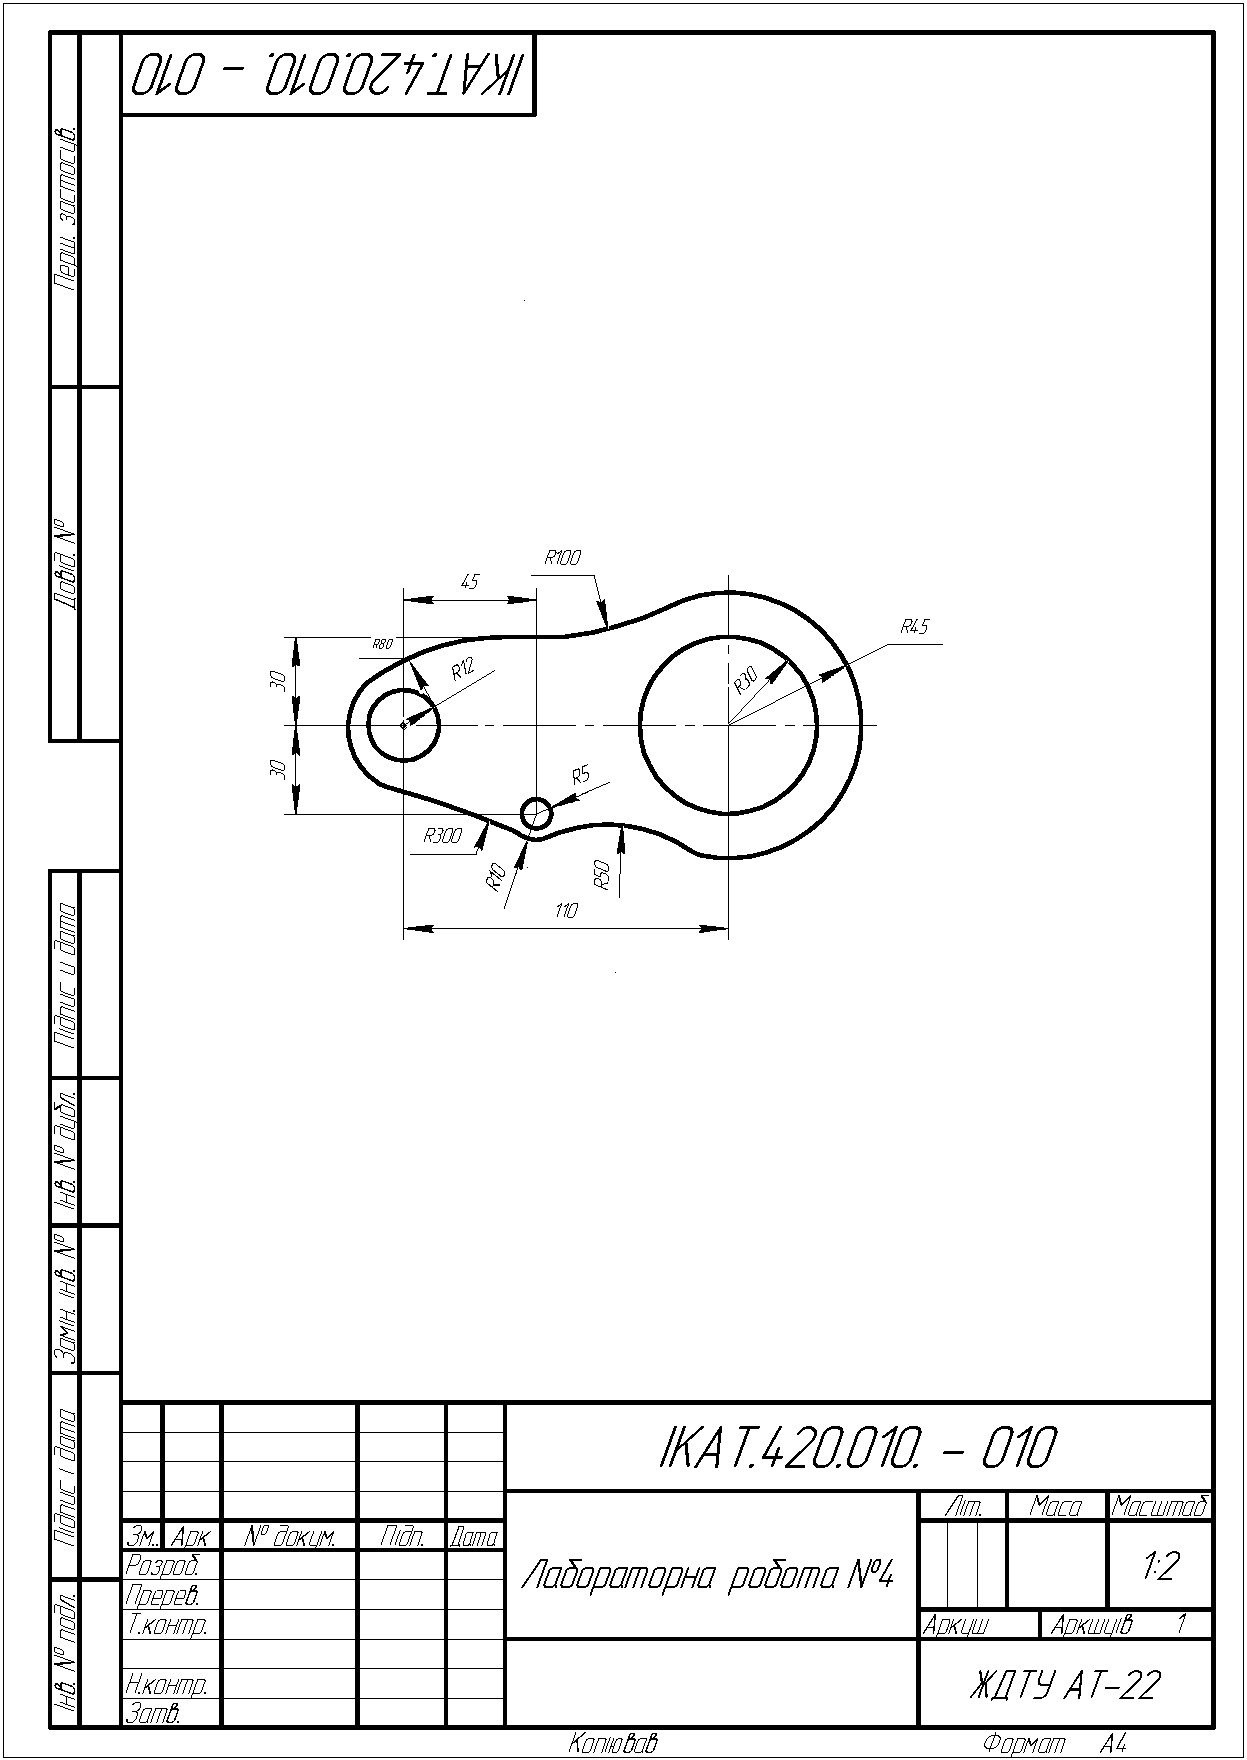
\includepdf{./src/lab4/drawing.pdf} \BorderText

\newpage
\section*{Висновок}

В ході виконання данох лабораторної роботи було вивичено особливості роботи програмою (а саме з
кривими та дугами) та побудовано задане за варіантом креслення деталі.
